\newpage

\begin{figure}[h!]
\centering
\scalebox{1}{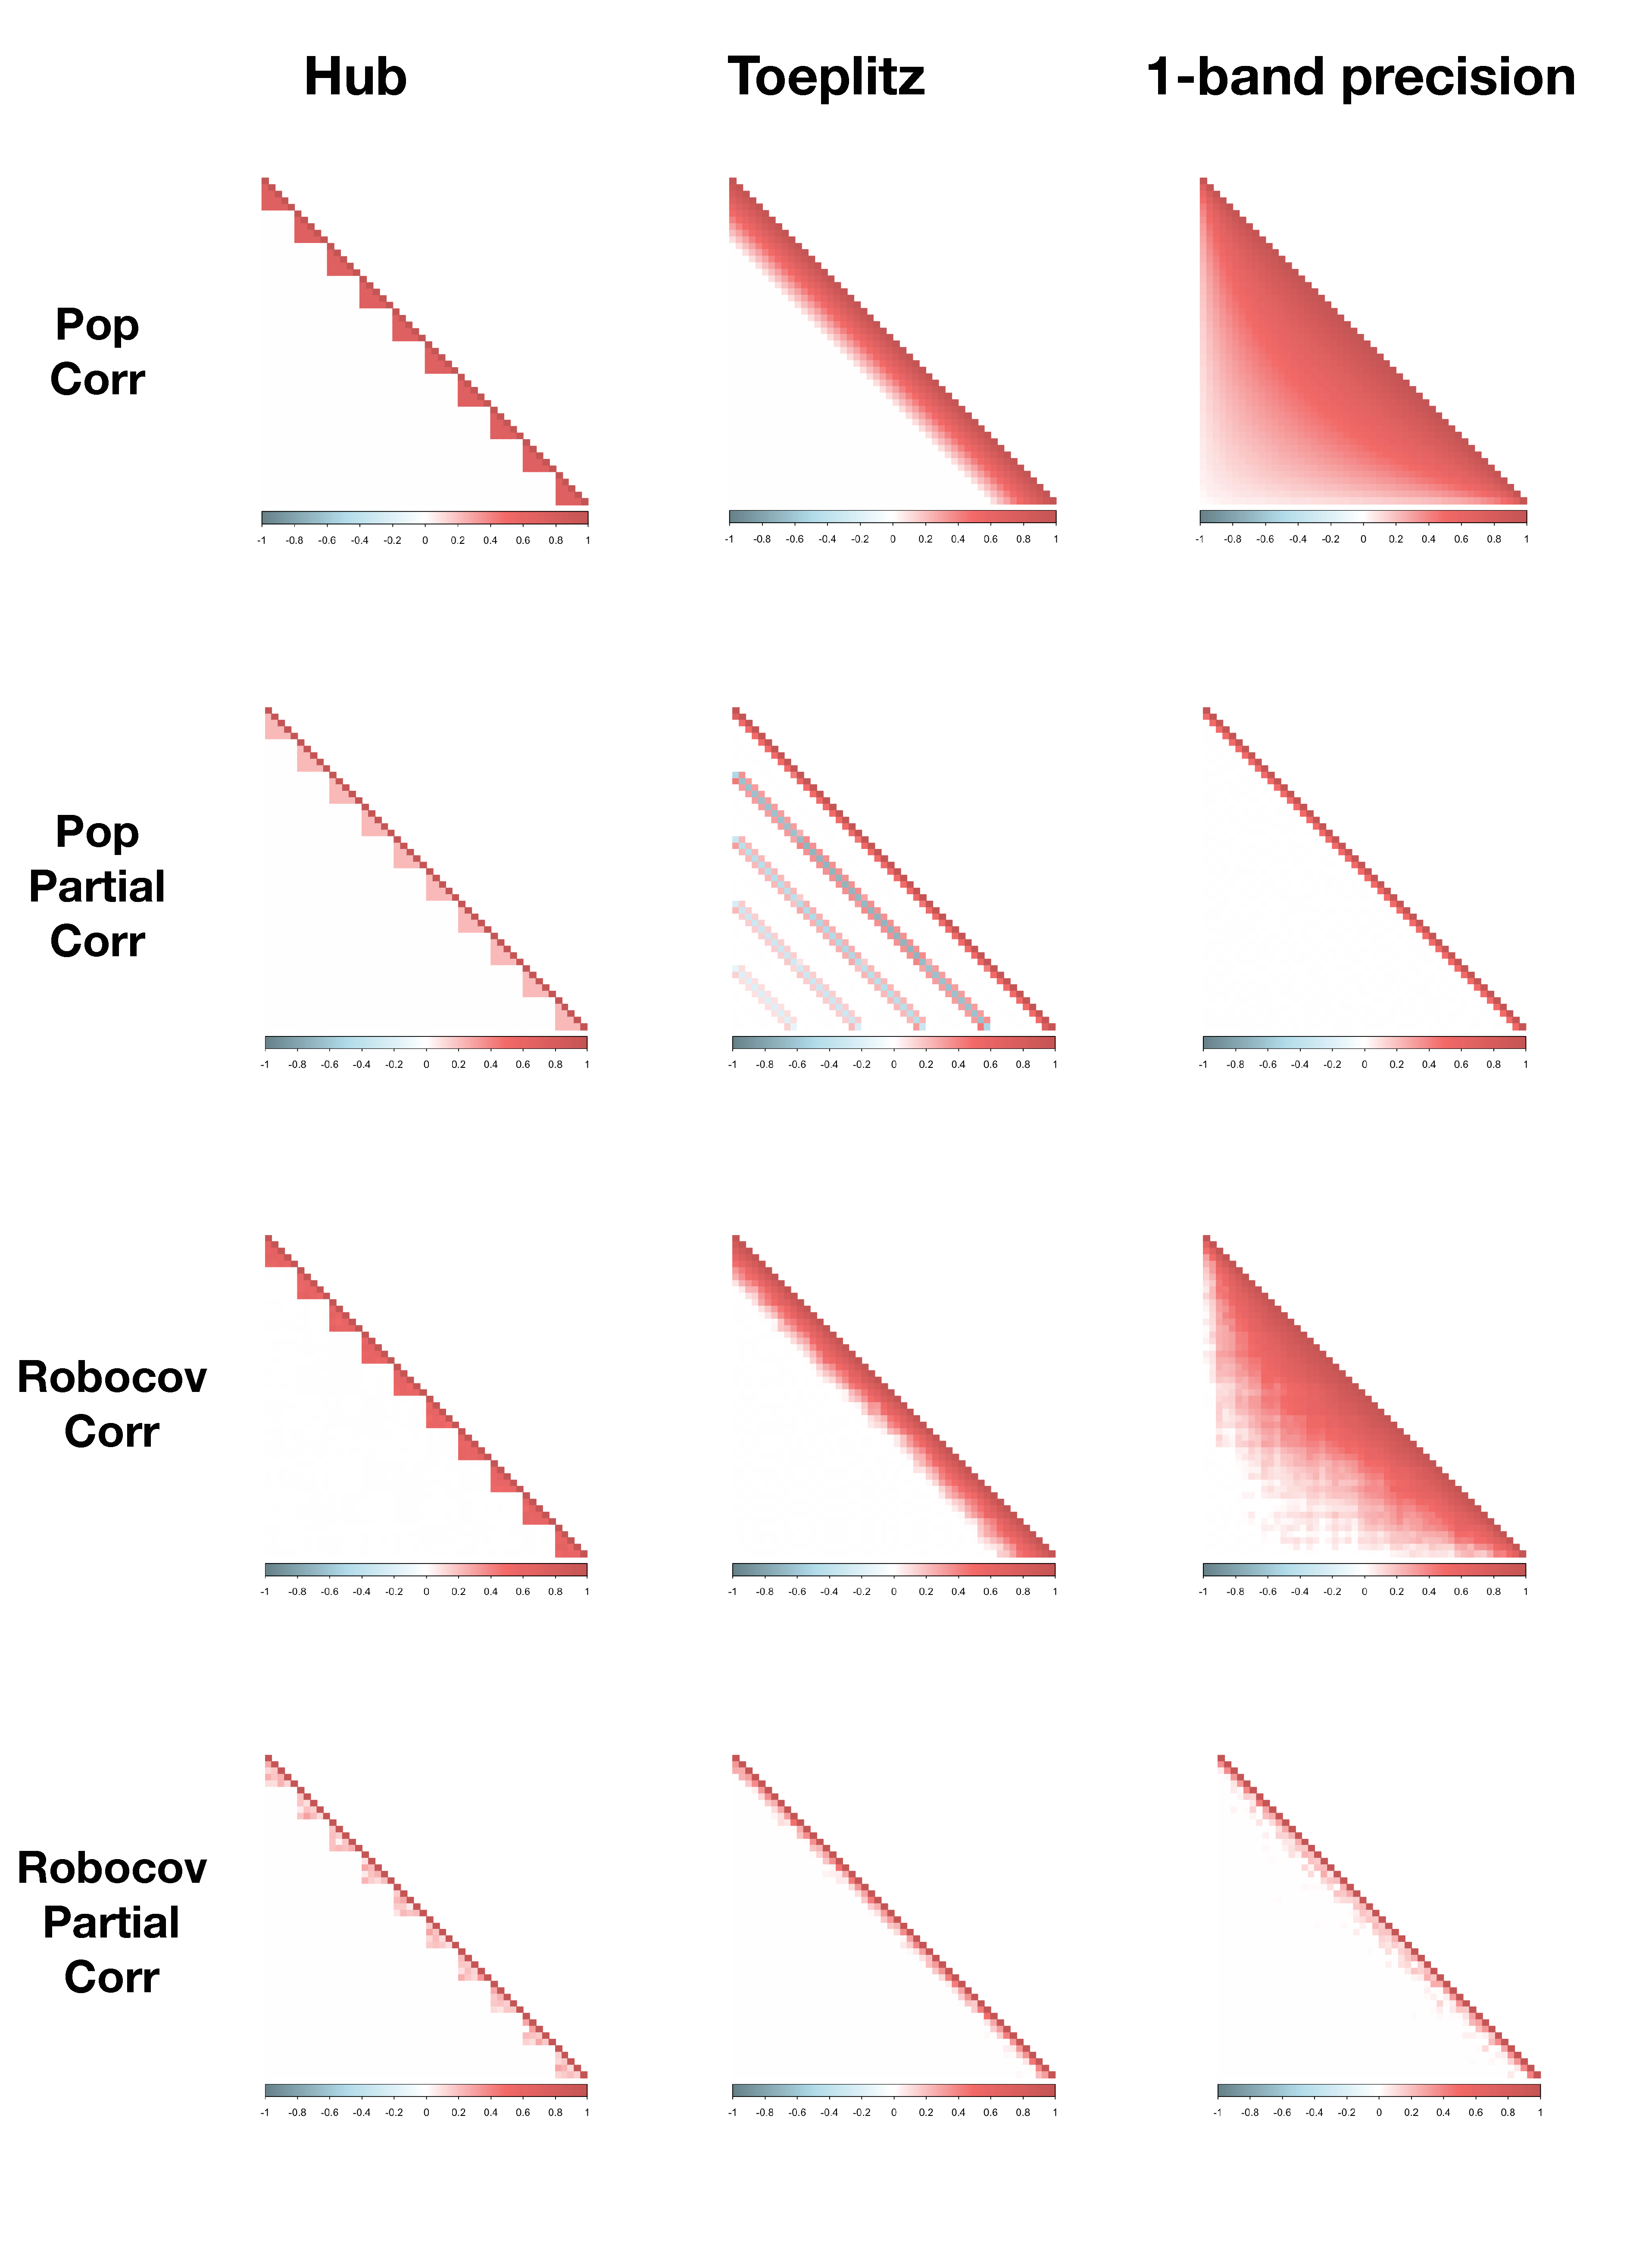
\includegraphics[width=\textwidth]{figures/Figure1_eps}}
\caption{\small {\textbf{Simulation results of applying \Robocov{} correlation and partial correlation estimators on Hub, Toeplitz and 1-band precision correlation structures}: We applied \Robocov{} correlation and partial correlation estimators on data generated from Hub, Toeplitz or 1-band precision matrix based population models (see Simulation settings in Supplementary Note) with $N=500$ samples, $P=50$ features and $\pi=0.5$ proportion of missing data. We present the population correlation matrix in the first row, population partial correlation matrix in second row, \Robocov{} correlation matrix in third row and \Robocov{} partial correlation matrix in last row. The tuning parameter for \Robocov{} correlation matrix (and partial correlation matrix) estimation was determined by cross-validation.}}
\label{fig:sim_results}
\end{figure}

\newpage
\begin{figure}[h!]
\centering
\scalebox{1}{\includegraphics[width=\textwidth]{figures/Figure1a_eps}}
\caption{\small {\textbf{Illustrative examples of pairwise sample correlation estimator, \Robocov{} correlation and partial correlation estimators for 2 genes}:
(Left column)  \textbf{ARHGAP30} gene and (Right column) \textbf{GSTM1} gene. Each column shows the (A) pairwise sample correlation estimator, (B) \Robocov{} correlation estimator and  (C) partial correlation estimator stacked from top to bottom.}}
\label{fig:gtex_demo}
\end{figure}


\newpage
\begin{figure}[h!]
\centering
\scalebox{0.85}{\includegraphics[width=\textwidth]{figures/Figure2_eps}}
\caption{\small {\textbf{Examples of genes with high average \Robocov{} correlation across all tissue pairs but with distinct expression profiles}: (A) \textbf{RPL9} gene has uniformly high TPM (transcripts per million) values across most tissues (inset picture). (B) \textbf{HBB} shows high expression specifically in Whole Blood (inset picture). The expression profile plots for the genes have been fetched from the GTEx Portal (\url{https://gtexportal.org/home/}).}}
\label{fig:gtex_examples_main}
\end{figure}

\newpage
\begin{figure}[h!]
\centering
\scalebox{0.8}{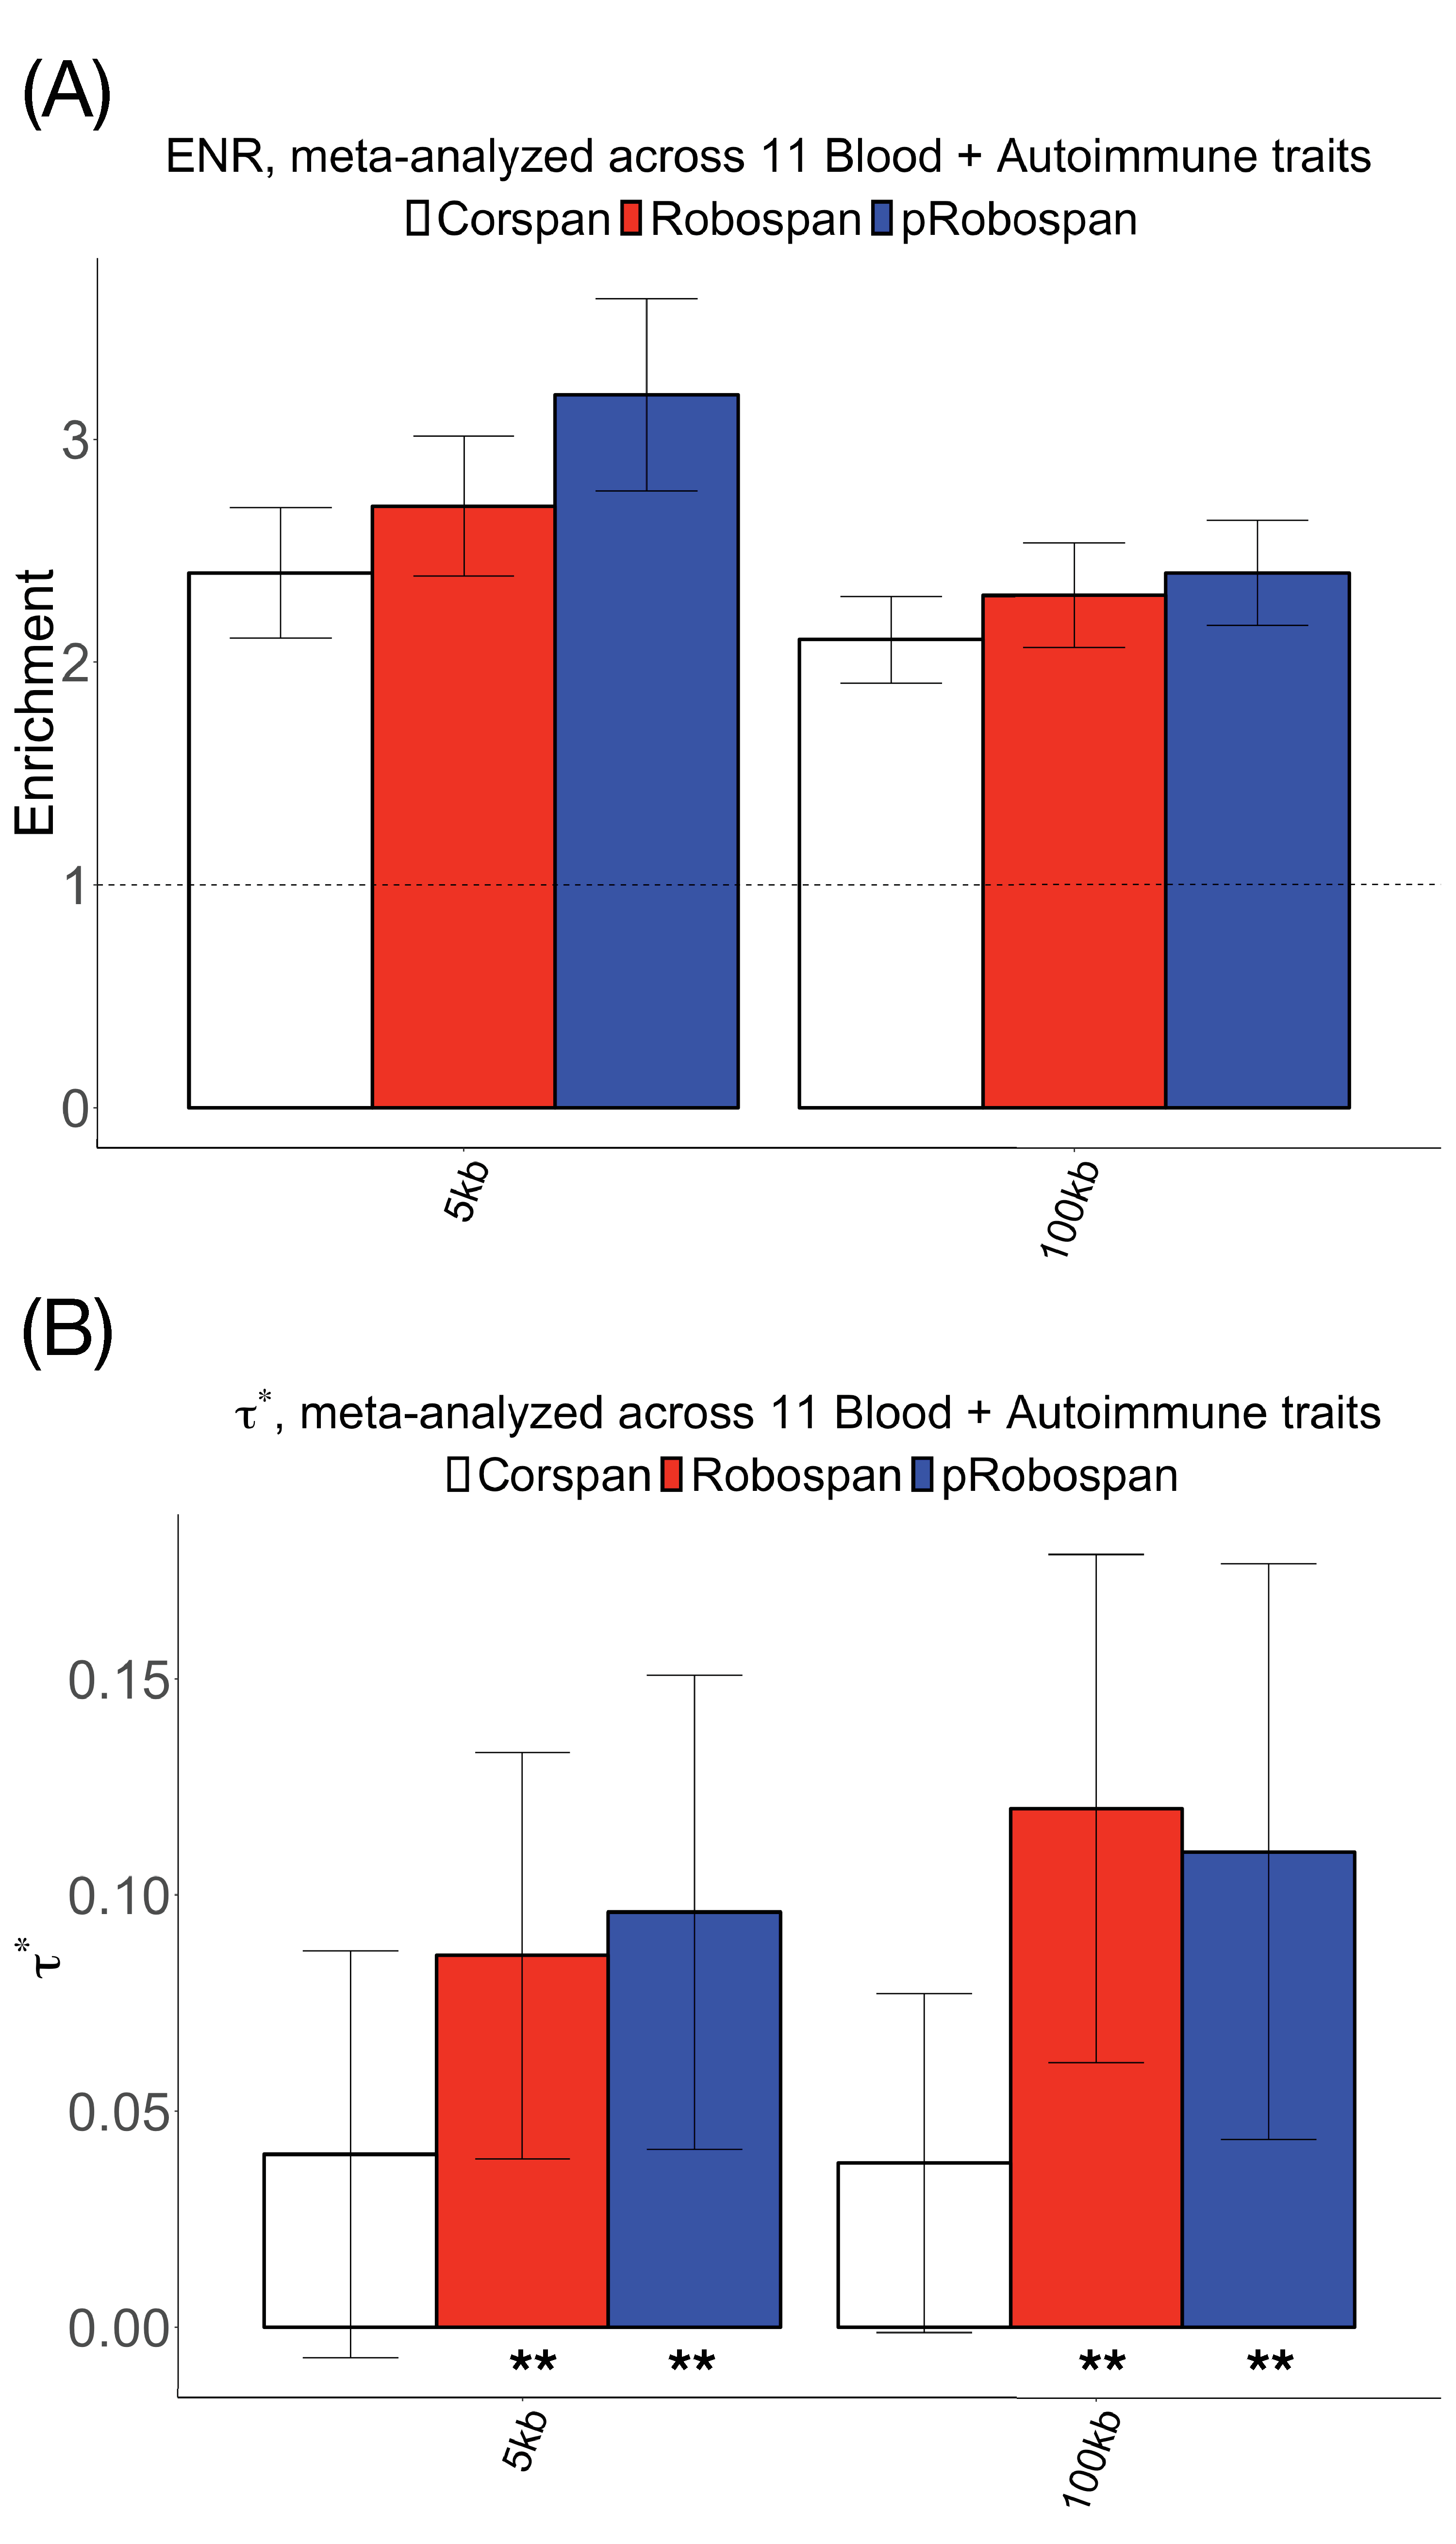
\includegraphics[width=\textwidth]{figures/Figure3_eps}}
\caption{\small {\textbf{Disease informativeness of 5kb and 100kb SNP annotations for \Corspan{}, \Robospan{} and \pRobospan{} gene sets}: (A) Heritability enrichment, conditional on baseline-LD model (v2.1). The base enrichment level is 1. (B) Standardized effect size ($\tau^{\star}$) conditional on baseline-LD model for \Corspan{} (left column, white), \Robospan{} (middle column, red) and \pRobospan{} (right column, blue) gene sets. Results are meta-analyzed across 11 blood and autoimmune traits. ** denotes annotations that are significant after Bonferonni correction ($P < 0.05/8$) where $8$ is the total number of SNP annotations tested. Error bars denote 95$\%$ confidence intervals. Numerical results are reported in Table \ref{tab:Robocov_marginal}.}}
\label{fig:Robocov_marginal}
\end{figure}

